\documentclass[useAMS,usenatbib]{mn2e}
\bibliographystyle{mnras}
\setlength{\bibhang}{2.0em}
\setlength\labelwidth{0.0em}
\setlength{\topmargin}{-1.2cm}

%\usepackage{times,psfig,epsfig} 
\usepackage{graphicx}%rotating, graphicx,dsfont}
\usepackage{xcolor}
\usepackage{amssymb,amsmath,bm}
\usepackage{hyperref}
\usepackage{bbm}
\usepackage{stmaryrd}
\usepackage[mathscr]{euscript} % caligraphic alternative
\usepackage{dsfont}
\usepackage{calrsfs}
\usepackage{textcomp}
%\usepackage{fourier} % screws format.
\usepackage{comment}
\usepackage[makeroom]{cancel}
\usepackage[export]{adjustbox}
\hypersetup{colorlinks=true,citecolor=blue}
% \usepackage[utf8]{inputenc}
%\usepackage{lipsum}
%\usepackage{pifont}
%\usepackage{balance}
\usepackage{multirow}
%\usepackage{widetext}

\hypersetup{
    colorlinks=false,
    citecolor=blue,
    linkcolor=blue,
    linktoc=page
}

\setcounter{tocdepth}{3}
\setcounter{secnumdepth}{3}

\newcommand{\aap}{Astron.\ Astrophys.\ }
\newcommand{\apj}{Astrophys.\ J.\  }
\newcommand{\apjl}{Astrophys.\ J.\ Lett.\  }
\newcommand{\apjs}{Astrophys.\ J.\ Suppl.\  }
\newcommand{\mnras}{Mon.\ Not.\ R.\ Astron.\ Soc.\ }
\newcommand{\na}{New Astronomy} 
\newcommand{\nat}{Nature} 
\newcommand{\npb}{Nucl.\ Phys.\ B} 
\newcommand{\physrep}{{\em Phys.\ Rep.}}
\newcommand{\pasj}{Publ.\ Astron.\ Soc.\ Japan\ }
\newcommand{\prd}{Phys.\ Rev.\ D\ }
\newcommand{\jcap}{Journal of Cosmology and Astro-Particle Physics}

\newcommand{\p}{\ensuremath{\partial}}
\newcommand{\del}{\ensuremath{\delta}}
\newcommand{\Del}{\ensuremath{\Delta}}
\newcommand{\lam}{\ensuremath{\lambda}}
\newcommand{\Lam}{\ensuremath{\Lambda}}
\newcommand{\gam}{\ensuremath{\gamma}}
\newcommand{\Gam}{\ensuremath{\Gamma}}
\newcommand{\sig}{\ensuremath{\sigma}}
\newcommand{\ep}{\ensuremath{\epsilon}}
\newcommand{\delc}{\ensuremath{\delta_{\rm c}}}
\newcommand{\nuc}{\ensuremath{\nu_{\rm c}}}
\newcommand{\epc}{\ensuremath{\epsilon_{\times}}}
\newcommand{\Sc}{\ensuremath{S_{\times}}}
\newcommand{\So}{\ensuremath{S_{0}}}
\newcommand{\delo}{\ensuremath{\delta_{0}}}
\newcommand{\delh}{\ensuremath{\delta_{\rm h}}}
\newcommand{\rhoh}{\ensuremath{\rho_{\rm h}}}

\newcommand{\Msun}{\ensuremath{M_{\odot}}}

\newcommand{\avg}[1]{\ensuremath{\left\langle \,#1\, \right\rangle}}
\newcommand{\etal}{et al.}

\newcommand{\der}{\ensuremath{{\rm d}}}
\newcommand{\dir}{\ensuremath{\delta_{\rm D}}}
\newcommand{\HT}{\ensuremath{\Theta_{\rm H}}}

\newcommand{\erfc}[1]{\ensuremath{{\rm erfc}\left(#1\right)}}
\newcommand{\erf}[1]{\ensuremath{{\rm erf}\left(#1\right)}}

\newcommand{\trp}{\ensuremath{{\rm Tr\,}\psi}}
\newcommand{\trz}{\ensuremath{{\rm Tr\,}\zeta}}
\newcommand{\tDL}{\ensuremath{\Delta\widetilde{\Lambda}}}
\newcommand{\tDl}{\ensuremath{\Delta\widetilde{\lambda}}}

\newcommand{\Xv}{ {\bf X}}

\newcommand{\tj}[6]{ \begin{pmatrix}
   #1 & #2 & #3 \\
   #4 & #5 & #6 
  \end{pmatrix}}
  
\newcommand{\nj}[9]{ \begin{Bmatrix}
   #1 & #2 & #3 \\
   #4 & #5 & #6 \\ 
   #7 & #8 & #9
  \end{Bmatrix}}

\newcommand{\sj}[6]{ \begin{Bmatrix}
   #1 & #2 & #3 \\
   #4 & #5 & #6 
  \end{Bmatrix}}

\newcommand{\cg}[6]{
C^{#1 #2}_{#3 #4 #5 #6}
}
  
\newcommand{\be}{\begin{equation}}
\newcommand{\ee}{\end{equation}}
\newcommand{\Cal}[1]{\ensuremath{\mathcal{#1}}}
\newcommand{\bea}{\begin{eqnarray}}
\newcommand{\eea}{\end{eqnarray}}
\newcommand{\bdm}{\begin{displaymath}}
\newcommand{\edm}{\end{displaymath}}
\newcommand{\de}{d}
\newcommand{\Om}{\Omega}
\newcommand{\rmd}{\textrm{d}}
\newcommand{\dc}{\delta_{cr}}
\newcommand{\vk}{{\bf k}}
\newcommand{\bfn}{\hat{\bf n}}
\newcommand{\mone}{$^{-1}$}
%\newcommand{\sqr}{$^2$}
\newcommand{\cub}{$^3$}
\newcommand{\flunits}{erg s$^{-1}$ cm$^{-2}$}
\newcommand{\ypar}{$y$-parameter}
\newcommand{\lcdm}{$\Lambda$CDM}
\newcommand{\lcdmn}{$\nu$\lcdm}
\newcommand{\omegam}{$\Omega_{\rm m}$}
\newcommand{\omegacdm}{$\Omega_{\rm CDM}$}
\newcommand{\omegal}{$\Omega_\Lambda$}
\newcommand{\omegab}{$\Omega_{\rm b}$}
\newcommand{\omeganu}{$\Omega_\nu$}
\newcommand{\fnu}{$f_\nu$}
\newcommand{\smnu}{$\Sigma \, m_\nu$}
\newcommand{\smnut}{$\Sigma \, m_\nu=0,\,0.17,\,0.3,\,0.53$ eV}
\newcommand{\sigmae}{$\sigma_8$}
\newcommand{\hzero}{$H_0$}
\newcommand{\subfind}{\textsc{subfind}}

\newcommand{\msun}{$M_{\odot}$} 
\newcommand{\mfiveh}{$M_{200}$}
\newcommand{\rfiveh}{$R_{200}$}
\newcommand{\yfiveh}{$Y_{200}$}
\newcommand{\hmone}{$\,h^{-1}$}
\newcommand{\hmthree}{$\,h^{-3}$}
\newcommand{\wmap}{{\it WMAP}}
\newcommand{\planck}{{\it Planck}}
\newcommand{\erosita}{{\it eROSITA}}
\newcommand{\spt}{SPT}
\newcommand{\act}{ACT}
\newcommand{\eps}{\epsilon_\times}
\newcommand{\rv}{r_v}
\newcommand{\Gb}{\frac{\Gamma^2}{\beta^2}}
\newcommand{\tilmu}{\tilde{\mu}}
\newcommand{\tilsig}{\tilde{\sigma}}
\newcommand{\mrm}[1]{\mathrm{#1}}

\def\fe{f_{\rm red}}
\def\lfs{\lambda_{\rm FS}}
\def\Ms{\, h^{-1} \, M_\odot}
\def\Mpc{\, h^{-1} \, {\rm Mpc}}
\def\Mpccube{\, h^{-3} \, {\rm Mpc}^3}
\def\Gpc{\, h^{-1} \, {\rm Gpc}}
\def\cGpc{\, h^{-3} \, {\rm Gpc}^3}
\def\kMpc{\, h \, {\rm Mpc}^{-1}}
\def\icMpc{\, h^3 \, {\rm Mpc}^{-3}}
\def\dk{\frac{\mathrm{d}^3\,k}{(2\pi)^3}\,}
\def\dr{\mathrm{d}^3\,r\,}
\def\dsa{\mathrm{d}^3\,s_1\,}
\def\dsb{\mathrm{d}^3\,s_2\,}

\def\sigm{\sigma_{mm}}
\def\sigc{\sigma_{cc}}
\def\sigem{\sigma_{8,mm}}
\def\sigec{\sigma_{8,cc}}
\def\RT{\text{RT}}

\newcommand{\eq}[1]{Eq.~(\ref{#1})}
\newcommand{\eqs}[2]{Eqs.~(\ref{#1},\ref{#2})}
\newcommand{\fig}[1]{Figure~\ref{#1}}
\newcommand{\figs}[2]{Figures~\ref{#1},\ref{#2}}

\newcommand{\vb}[1]{\mathbf{#1}}
\def\ie{{\em i.e.}~}
\def\eg{{{\em e.g.}~}}

%\def\gad{\textsc{Gadget}}
\def\halofit{\textsc{halofit}}
\def\camb{\textsc{CAMB}}
\def\class{\textsc{CLASS}}
\newcommand{\gadget}{\textsc{gadget}}
\newcommand{\gadgetthree}{\textsc{gadget-3}}

\newcommand{\MW}[1]{\emph{\color{blue}[MW: #1]}}
\newcommand{\EC}[1]{\emph{\color{red}[EC: #1]}}

\title[Spectral RSD as an isotropic observable]{A spectral formulation of full sky redshift-space clustering with variable selection}

\author[M. J. Wilson]
{M. J. Wilson$^{1,2}$\thanks{e-mail: mjwilson@lbl.gov}
 \\~\\
\footnotesize
\footnotesize
$^1$Lawrence Berkeley National Laboratory, One Cyclotron Road, Berkeley, CA 93720, USA\\
$^2$Berkeley Center for Cosmological Physics, University of California, Berkeley, CA 94720, USA\\
}

\begin{document}
\maketitle 

\begin{abstract}
This paper presents extensions of current RSD estimators, modelling and covariance estimates to the finite-angle, variable selection regime and presents evaluation methods that are seemingly maximally efficient based on the remaining symmetry of the problem -- statistical isotropy about the observer.  The implementation of this method for the Dark Energy Spectrosocpic Instrument is provided as a worked example, with the Bright Galaxy Survey taken as a future survey for which these effects will be a concern.
\end{abstract}

\section{Introduction}
Intro
\begin{equation}
  \vb{s} \equiv \vb{r} + f \ (\vb{u} \cdot \boldsymbol {\hat r}) \ \boldsymbol{\hat r}\,
\end{equation}
where $f$ is the linear growth factor and $\vb{u}$ is related to the peculiar velocity $\vb{v}$ and the Hubble parameter $H$, $\vb{v} =  aH f \vb{u}$. In linear theory, we can write the following relation between the redshift-space and real-space density field as %\citep{Kai87, H92, H98}.
\begin{equation}
\label{eq:RSD}
\delta_s(\vb{s}) = \left[1+ \beta \left(\nabla^2 - e^{-2 \rho} \left \{ \nabla^2_{\Omega} - \alpha(\vb{s}) \frac{\partial}{\partial \rho} \right \} \right) \nabla^{-2} \right] \delta(\vb{s}) \;,
\end{equation}
where $\rho = \ln s$ and $\alpha(\vb{s})$ is given by 
\begin{equation}
\alpha(\vb{s}) \equiv \frac{\der}{\der \rho} \ln \bar n(s).
\end{equation}
Here $\bar n(s)$ is the true (configuration-space) number density evaluated at the redshift-space position; No attempt has been made to account for the effect on the observed selection function from RSD.  If the number density is approximated by a local power law, $\bar n \propto s^n$, then $\alpha(s)$ simply measures the slope.  As the radial distortion operator commutes with the angular momentum operator, the eigenmodes of the latter -- of which the spherical harmonics are a representation -- are also eigenmodes of the distortion operator; This is a consequence of the remaining statistical isotropy about the observer.  We show below that a constant $\alpha$ of zero may be assumed at this stage, and therefore the problem is distortion operator is scale free (Hamilton and Culhane 1997), although this is not the case for the real-space density field.  A natural radial distance metric is logarithmic in a scale-free case; as $\partial / \partial \rho$ commutes with the distortion operator, it completes the set of commuting operators.  A basis may be formed from the product of the eigenfunctions of these operators.   Fig.~\ref{fig:triangle} shows the geometry of the problem.  
\begin{comment}
\begin{figure}
\begin{center}
\begin{picture}(250,250)
\Large
\thicklines
\qbezier(125.0,0.0)(125.0,112.5)(125.0,218.8)
\qbezier(125.0,0.0)(156.2,125.0)(187.5,250.0)
\qbezier(125.0,0.0)(93.8,93.8)(62.5,187.5)
\qbezier(62.5,187.5)(125.0,218.8)(187.5,250.0)
\thinlines
\multiput(125,219)(0,6){5}{\line(0,1){3}}
\put(110,60){$\displaystyle{\frac{\theta}{2}}$}
\put(128,60){$\displaystyle{\frac{\theta}{2}}$}
\put( 70,120){$\vec{s}_1$}
\put(160,120){$\vec{s}_2$}
\put(130,180){$\vec{d}$}
%\put( 70,182){\rotatebox{27}{$s(1-t)$}}
%\put(160,227){\rotatebox{27}{$st$}}
\put(115,205){$\phi$}
\put(160,250){\vector(-2,-1){75}}
\put(110,230){$\vec{s}$}
\end{picture}
\caption{The assumed geometry and angles.  The two galaxies lie at $\vec{s}_1$
and $\vec{s}_2$, with separation vector $\vec{s}=\vec{s}_1-\vec{s}_2$ and
enclosed angle $\theta$.
We take the line of sight to be parallel to the angle bisector, $\vec{d}$,
which divides $\vec{s}$ into parts of lengths $st$ and $s(1-t)$.  The
separation vector, $\vec{s}$, makes an angle $\phi$ with the line of sight
direction, $\hat{d}$. \label{fig:conf}}
\end{center}
\label{fig:triangle}
\end{figure}
\end{comment}

\begin{figure}
    \centering
    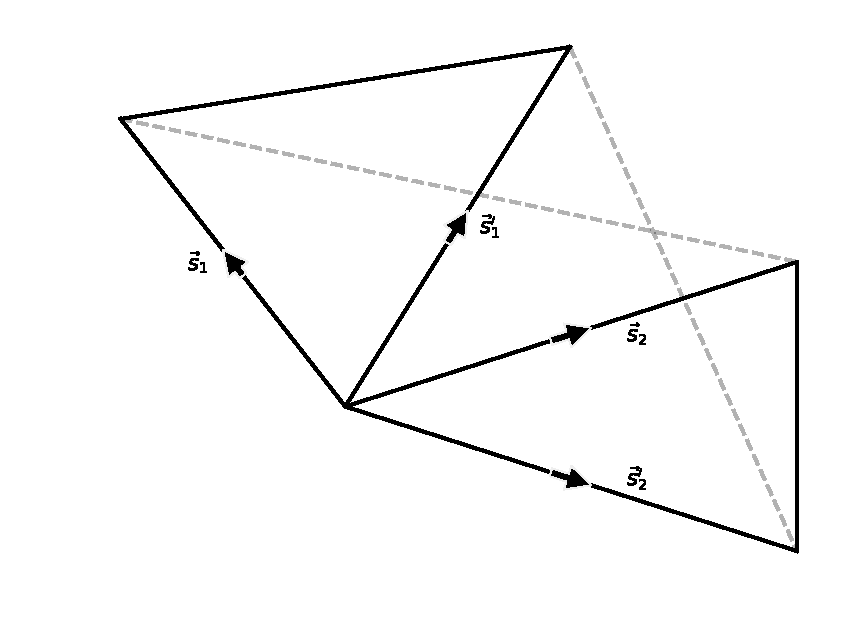
\includegraphics[scale=0.6]{triangle.pdf}
    \caption{The geometry.}
    \label{fig:triangle}
\end{figure}


\section{The finite-angle redshift-space correlation function}
As observers, we count pairs of galaxies whose locations are defined by $\vb{s}_1$ and $\vb{s}_2$, with separation $\vb{s} = \vb{s}_1 - \vb{s}_2$ .  In redshift space, the correlation function -- the expected pair count above random -- for finitely separated pairs can be decomposed as  
\begin{align}
&\xi_s(\boldsymbol s, \boldsymbol d) \ = \ (4 \pi)^{3/2} \ i^{-n} \ (-1)^{\ell_1} 
 \  \frac{\tilde \alpha^n_{\ell_1, \ell_2}(s_1, s_2) \ \tilde \beta^n_{\ell_1, \ell_2}}{\sqrt{(2 \ell_1 +1)(2 \ell_2 + 1)}} \notag \\ & \quad \times \sum_{L=|\ell_1 - \ell_2|}^{\ell_1 + \ell_2} (-i)^L \sqrt{2L+1}  \tj{\ell_1}{\ell_2}{L}{0}{0}{0} \int_{\ln k}  \mathcal{A}^{n}_L(k) \ j_L(ks) \ T_{\ell_1 \ell_2 L} (\blacktriangle)
\end{align}
in \emph{linear theory};  See eqn. (7) of Szalay (1997) and eqn. (4) of Szapudi (2004)\footnote{Using the notation V163(7) to denote eqn. (7) on pg. 163 of Varshalovich, V163(7) allows the removal of the asymmetric $(-1)^{\ell_2}$ term from this original Szalay expression.}.  Here an Einstein summation over $n, \ell_1$ and $\ell_2$ is implied; In total, there are six terms in the absence of RSD-selection mixing and fourteen terms with incomplete selection as $(\ell_1~+~\ell_2~+~n)$ must be even for $\xi_s$ to be real.  Here the triangle formed by a pair is specified by the (scalar) separation, $s$, and the shape, $\blacktriangle \equiv (\boldsymbol {\hat s}, \boldsymbol {\hat s}_1, \boldsymbol {\hat s}_2)$;  This is an abstraction for the physical $\xi_s$ that removes the constraint placed on $\blacktriangle$ by $s$; see Appendix A.  For simplicity, we neglect terms due to Poisson sampling and higher-order biasing by considering only the correlation of dark matter.  The former should be legitimate for the highly complete BGS survey we consider, but the inclusion of Poisson sampling should be straightforward.  Moreover, there is unlikely to be a strong mixing with the large scale effects that are our focus, as the variance due to mode sampling dominates in this regime.  

When defined in this manner, the form is separable with respect to the real-space cosmology, $\xi^{n}_L(s)$, redshift-space cosmology, $\beta^{n}_{\ell_1 \ell_2}$, selection, $\tilde \alpha^{n}_{\ell_1 \ell_2}$, and finite-angle effects, $T_{j_1 j_2 J}(\blacktriangle)$;  For instance, $\tilde \beta^2_{1, 1} = \beta^2$ and $\tilde \alpha^2_{1,1} = \alpha(s_1) \ \alpha(s_2)$.  It is common practice to neglect the two penultimate dependencies, which may lead to systematic error for current and future surveys.  Here, the basis in solid angle is 
\begin{align}
&T_{\ell_1 \ell_2 L}(\blacktriangle) \notag \\ 
&\equiv 
\{ Y_{\ell_1} (\Omega_1) \otimes \{ Y_{\ell_2} (\Omega_2) \otimes Y_{L} (\Omega_3)\}_{\lambda_1} \}_{00}
& \notag \\
&\equiv (-1)^{\ell_1 + \ell_2 + L} \ \delta^{K}_{\lambda \ell_1} \notag \\ 
& \quad \times \sum_{m_1 m_2 M} \tj{\ell_1} {\ell_2}{L}{m_1}{m_2}{M} 
\ Y_{\ell_1 m_1}(\boldsymbol {\hat s}_1)
\ Y_{\ell_2 m_2}(\boldsymbol {\hat s}_2)
\ Y_{L M}(\boldsymbol {\hat s})
\end{align}
and the coefficient associated to the expansion in eigenfunctions of separation is 
\begin{align}
\mathcal{A}^{n}_L(k) &\equiv \int s^2 \ ds \ \xi^{n}_L(s) \ j_L(ks) \notag \\ &= k^{-n} \Del^2(k),
\end{align}
where $\xi^n_L(s)$ has been defined by Szapudi (2004).  Here the basis in spherical Bessel functions has resulted from a Fourier Transform of $\xi_s$, that has a further rotational symmetry even in the finite-angle regime, e.g.  about the line of sight.   

To the extent that the real-space density field is also scale free, $\Del^2(k) \propto k^m$, then the separation dependence:
\begin{equation}
    \int_{\ln k} \mathcal{A}^{n}_L(k) \ j_L(ks) = \left ( \frac{\pi}{2} \right ) \ U_{L + \frac{1}{2}} \left (m - n + \frac{1}{2} \right ) \ e^{-(m-n-2) \rho},
\end{equation}
maps succinctly to a finite number of scale-free power laws; $U$ is defined by eqn. (172) of Hamilton (2000). This illustrates the strength of a well-chosen basis, which corresponds to the logarithmic plane waves of Hamilton and Culhane (1997) in this case.  In this representation, 
\begin{equation}
    k^{-n} \Del^2(k) = k^\gamma
    \int \frac{d \omega}{(2 \pi)} \ \tilde \Del^2_n(\omega) \ e^{i \omega \ln k}
\end{equation}
and, more generally, the structure in separation is represented by complex power laws:
\begin{align}
    &\int \mathcal{A}^{n}_{L}(k) \ j_L(ks) \ d \ln k = \notag \\ 
    & \int \frac{d\omega}{\sqrt{8\pi}} \  U_{L+\frac{1}{2}} \left (-\frac{1}{2} + \gamma + i \omega \right ) \ \tilde \Del^2_n(\omega) \ e^{-(1 + \gamma + i\omega) \rho},  
\end{align}
where the scale-free nature of the basis is apparent.  %The simplification for a featureless $\Del^2(k)$ is due to the mean (logarithmic) mode being purely real. 
Due to both the M\'esz\'aros effect and Baryon Acoustic Oscillations, there are preferred scales in the real-space spectrum.  As such this does not reduce to simply a finite number of powerlaws, but, to the extent that the dynamic range of the bandwidth in $\omega$ is smaller than that in $k$, this is a more efficient representation.  % Due to the rotational symmetry about the line of sight and scale-free nature of the distortion operator, perhaps the most natural basis for separation are spherical Bessel functions in $\rho$.

While the $T_{\ell_1 \ell_2 L} (\blacktriangle)$ are a subset of the Tripolar Spherical Harmonics -- a complete orthonormal basis for functions that depend on three vectors (poles).  Under a rotation defined by the three Euler angles, the Tripolar Spherical Harmonics transform akin to any irreducible tensor: 
\begin{align}
&\hat D(\alpha, \beta, \gamma)  \ \{ Y_{\ell_1} (\Omega_1) \otimes \{ Y_{\ell_2} (\Omega_2) \otimes Y_{\ell_3} (\Omega_3) \}_\lambda \}_{LM'} =  \notag \\ 
& \sum_{M} D^L_{M M '}(\alpha, \beta, \gamma) \{ Y_{\ell_1} (\Omega_1) \otimes \{ Y_{\ell_2} (\Omega_2) \otimes Y_{\ell_3} (\Omega_3) \}_\lambda \}_{LM},      
\end{align}
where $D^L_{M M '}(\alpha, \beta, \gamma)$ is the Wigner rotation matrix.  Due to the remaining symmetry of finite-angle RSD -- statistical isotropy about the observer -- $\xi_s$ must be comprised solely of the rank-zero, $(L,M, \lambda) = (0,0, \ell_1)$, Tripolar Spherical Harmonics, which remain invariant under global rotations of the coordinates; This subset may be labelled as $T_{\ell_1 \ell_2 L}(\boldsymbol {\hat s}, \boldsymbol {\hat s}_1, \boldsymbol {\hat s}_2)$, as above.  Given that $(\ell_1 + \ell_2 + L)$ must be even for the Wigner-3j in eqn. (4) to be non-zero, $T_{\ell_1 \ell_2 L}(\blacktriangle)$ is invariant under permutations of columns -- see V244(5) -- and therefore $1 \leftrightharpoons 2$. 

For small $s$, the Kaiser plane-parallel limit is recovered with $\boldsymbol {\hat s_1} \simeq \boldsymbol {\hat s_2} \simeq \boldsymbol {\hat d}$ and the usual Hamiltonian multipoles are complete according to eqn. (3) and (10) of Szapudi (2004); This follows from
\begin{align}
T_{\ell_1 \ell_2 L}(\blacktriangle) \simeq & \ (-1)^{\ell_1 + \ell_2 + L} \sqrt{\frac{(2\ell_1 +1)(2\ell_2+1)(2L+1)}{(4 \pi)^3}} \notag \\ 
& \times \tj{\ell_1}{ \ell_2}{L}{0}{0}{0} \  \mathcal{L}_{L}(\boldsymbol {\hat s}_1 \cdot \boldsymbol {\hat s}).
\end{align}
for $\boldsymbol {\hat s_1} \simeq \boldsymbol {\hat s_2}$.

\section{Two-point redshift-space likelihoods}
\label{sec:twopoint_estimators}
Current RSD analyses extend the Kaiser model to the curved sky by defining the $A^{\rm th}$ power spectrum multipoles as an integral over pairs with the line of sight taken to be either the angle bisector or midpoint, rather than a global $\boldsymbol{ \hat z}$ axis.  This leads to the Yamamoto estimator \citep{Yam06}:
\begin{align}
\label{eq:PkY}
  \hat{P}_A^Y(k) \equiv (2A +1) \int \mathrm{d}^3 s_1 \ \mathrm{d}^3 s_2\ \delta(\vb{s}_1) \ \delta(\vb{s}_2) \int_{\boldsymbol {\hat k}} \ e^{-i\vb{k} \cdot \vb{s}} \ \mathcal{L}_A\left(\boldsymbol {\hat k} \cdot \boldsymbol {\hat d} \right),
\end{align}
for 
\begin{align}
\int_{\boldsymbol{ \hat k}} & \equiv \int \frac{\mathrm{d} \Omega_\vb{k}}{4\pi}  \qquad \qquad
\int_{\boldsymbol s}^{\boldsymbol k} & \equiv  \int d^3s \ e^{-i\vb{k}\cdot \vb{s}}.
\end{align}
Unfortunately, while mitigating the more erroneous problems caused by assuming a global line of sight $\boldsymbol {\hat z}$, for the finite number of integer $A \in \{ 0, 2, 4 \}$ commonly assumed, this does nothing to account for the added structure of the finite-angle correlation function beyond the Kaiser plane-parallel limit;  This is simply due to the fact that the radial velocity for each galaxy is not equal to the other, nor equal to the component along the bisector (or midpoint) when $s$ and $\theta$ are large.  For practical reasons, often the line-of-sight to a pair member, e.g. $\boldsymbol {\hat s}_1$, is taken to be a proxy for $\boldsymbol {\hat d}$, which allows for efficient Fast Fourier Transform evaluations but leads to systematic error.  We refer to this as the endpoint approximation.     

Nevertheless, this defines a set of $\boldsymbol{ \hat k}$ averaged, $k$ dependent, statistics from which a likelihood may be formed.  It is neither complete, nor optimal, for a finite number of integer $A$.  As
\begin{equation}
\int_{{\boldsymbol {\hat k}}}^{ \boldsymbol s} \mathcal{L}_A \left(\boldsymbol {\hat k} \cdot \boldsymbol {\hat d} \right) =
\ i^A \ j_A(ks) \ \mathcal{L}_A \left(\boldsymbol {\hat s} \cdot \boldsymbol {\hat d} \right ),
\end{equation}
these $k$ dependent statistics are effectively obtained by weighting pairs according to the right hand side of eqn.~(11);  From the introduction, it is clear that this is simply an extraction of the independent (plane-parallel) coefficients via orthogonality;  Whereas the correlation function moments represent an incomplete extraction that returns a linear superposition of radial eigenfunctions.  This illustrates the sole, but important, difference between a power spectrum and correlation function approach.  In particular, the scale and $\boldsymbol {\hat s}$ dependence of the pair weighting is separable, as makes intuitive sense given eqn.~(4);  Fundamentally, this is a consequence of the preferred scale isolated by the $\nabla^{-2}$ common to both the linear and spherical distortion operators; see Hamilton and Culhane (1997).  In the following we generalise this effective pair weighting to one that accounts for the added structure for finite angles.


\subsubsection{A complete inclusion of finite-angle effects}
To form a practical likelihood, clearly a compression of $\xi_s(s, \blacktriangle)$ over the configuration is necessary.  From Section 2.1, it is clear that the Tripolar expansion coefficients yield the necessary physical information.  These may be obtained on the basis of the Tripolar Spherical Harmonic orthogonality:
\begin{align}
\Xi_{j_1 j_2 J}(s) &= \int_{\boldsymbol {\hat s}_1, \boldsymbol {\hat s}_2,  \boldsymbol {\hat s} | s} \xi_s(s, \blacktriangle) \ T^{*}_{j_1 j_2 J}(\blacktriangle) \notag \\ 
&= %(-1)^{\ell_2}% 
\ (4 \pi)^{3/2} (-1)^{j_1 + J} \ i^{J-n} \ \tilde{\beta}^{0}_{j_1 j_2} \notag \\ &\times \sqrt{\frac{2J+1}{(2 j_1 + 1)(2 j_2 + 1)}} \tj{j_1}{j_2}{J}{0}{0}{0} \ \xi^{0}_J(s),   
\end{align}
\begin{figure}
    \centering
    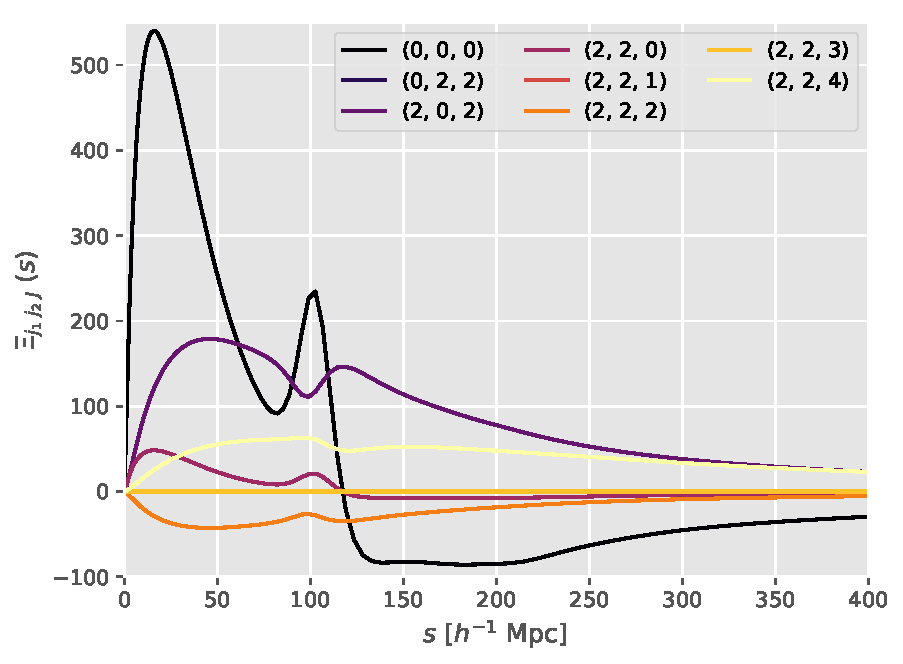
\includegraphics[scale=0.55]{XI.pdf}
    \caption{Wide-angle correlation functions.}
    \label{fig:XI}
\end{figure}
where the latter is true in the absence of RSD-selection mixing, i.e when $\bar n_s \propto (1/s^2)$ and the sum over $(n, \ell_1, \ell_2)$ reduces to four terms for which $n=0$ and $\alpha^{0}_{\ell_1 \ell_2}$ are unity; The apparent overcounting of the degrees of freedom for the configuration should be interpreted as an integral over all possible pairs and an abstraction for $\boldsymbol{\hat s}$ that releases it from the restriction placed by $s$.  For further discussion, see Appendix A.  Here, we have used that \smash{$T^{*}_{j_1 j_2 J}(\blacktriangle) = (-1)^{j_1 + j_2 + J} \ T_{j_1 + j_2 + J}(\blacktriangle)$}, where the prefactor is unity for those applicable to RSD.  It should be clear from the above section that this reduces to a linear combination of the Kaiser multipoles for small $s$.  By analogy to this limit, a Hankel transform,
\begin{equation}
F_{j_1 j_2 J}(k) = \mathcal{H} \left ( \Xi_{j_1 j_2 J}(s) \right ) \equiv \int s^2 ds \ j_J(ks) \ \Xi_{j_1 j_2 J}(s),
\end{equation}
yields 
\begin{align}
F_{j_1 j_2 J}(k) &= (-1)^{j_1 + J} \ i^{J-n} \ \tilde{\beta}^{0}_{j_1 j_2} \notag \\ &\times \sqrt{\frac{2J+1}{(2 j_1 + 1)(2 j_2 + 1)}} \tj{j_1}{j_2}{J}{0}{0}{0} \ \frac{P(k)}{\sqrt{4 \pi}}.
\end{align}
given $n=0$ and the Spherical Bessel function orthogonality relation, 
\begin{equation}
\int ds s^2 j_L (ks) \ j_L(qs) = \frac{\pi}{2 q^2} \ \delta^{K}(k-q).
\end{equation}
Here $P(k)$ is the isotropic real-space spectrum; i.e. specifying a $(j_1, j_2)$ pair selects a given $\beta_{j_1, j_2}$ factor which has a unique polynomial dependence on $\beta$; there are a number of such statistics labelled by $J$ -- those which satisfy the triangular inequality -- that may be optimally combined without loss.  

Analogously to the plane-parallel limit, this spectral representation picks out a given scale of the real-space power spectrum; Standard inflation typically predict this to be uncorrelated.  Thus the correlation is reduced between estimates on different scales, which is the principal advantage over configuration-space statistics on large scales.  In principle, with highly precise estimates, these additional statistics to the Kaiser multipoles on large scales are useful in breaking degeneracies with the other fitting parameters.  On small scales, where finite-angle effects are unimportant, these smoothly reduce to a linear combination of the complete Kaiser multipoles. 

%\subsection{Relation to Spherical-Bessel transform}

\subsection{A practical estimator}
Using eqn. (12), this weighting is 
\begin{equation}
\hat F_{j_1 j_2 J}(k) = \int_{\boldsymbol {s}_1, \boldsymbol {s}_2} \ j_J(ks) \ T^{*}_{j_1 j_2 J}(\blacktriangle) \ \delta(\boldsymbol {s}_1) \ \delta(\boldsymbol {s}_2), 
\end{equation}
in practice.  From eqn. (11) it is clear that this is simply the Yamamoto estimator when the configuration dependent factor of the pair weighting, $\mathcal{L}_J(\boldsymbol {\hat s} \cdot \boldsymbol {\hat d})$, is replaced by $T^{*}_{j_1 j_2 J}(\blacktriangle)$ for pairs with large separation.  The weighting to be applied is a product of the eigenfunctions of the three operators that commute with the radial distortion operator.

Eqn. (8) shows that the endpoint estimator is sufficiently precise to provide estimates free of systematic error for large $k$.  From the non-zero $J \in \{ 0,2,4\}$ estimated, $\hat F_{\j_1 j_2 J}(k)$ may be constructed with the appropriate Wigner-3j symbol.  For sufficiently small $k$, we know these to be both inexact and incomplete. But on these scales shot-noise is negligible and the catalogue of galaxies may be thinned by a large factor without loss of precision\footnote{Current surveys are designed to be shot noise limited at $q~\simeq~0.1 h^{-1} \rm{Mpc}$  ($\bar n P_{0.1} \simeq 1$). Given the ratio of the matter power spectrum at this scale to that at $q\simeq 0.01 \rm{Mpc} / h$, the catalogue may be thinned by around an order of magnitude.}.  With this reduced catalogue, the correction between a proper $T_{j_1 j_2 J}(\blacktriangle)$ and the Yamamoto weighting may be calculated starting with the pairs of largest separation; As the number of pairs to be counted goes as the thinning factor squared this is a large reduction in the required calculation.  At a given scale, these 
corrections will be found to be negligible and the pair counting may be ceased;  We anticipate this scale to be large, but not infinite.  Finally, these corrections are to be applied to the ${F^{\rm{end}}}_{j_1 j_2 J}(k)$ estimates to form an accurate input for the likelihood calculation.

Moreover, as eqn. (16) is simply the Hankel transform of the $T(\blacktriangle)$ weighted pairs as a function of separation, no explicit weighting by $j_L(ks)$ must actually be applied:  this may simply be achieved by applying the FFTlog algorithm (Hamilton 2000) to the weighted pair counts.  This is beneficial both as Spherical Bessel functions are slow to compute and because $\hat F_{j_1 j_2 J}(k)$ is then returned for all $k$ on a discrete grid in one FFT (and a weighted inverse).  Accounting for the systematic bias in this estimator due to absent pairs is  presented in Section 4.2. \emph{Is this shot noise free by construction?}.

\subsection{Endpoint $\xi_s$ moments by FFT}
A FFT estimator may also be employed in configuration space.  Consider the weighted number density, $\bar n_w(\mathbf{s})$, with Fourier transform 
\begin{equation}
    \tilde n_w(\mathbf{k}) = \int_{\boldsymbol s} e^{-i \boldsymbol {k} \cdot \boldsymbol s} \ \bar n_w(\mathbf{s}).
\end{equation}
The $GR$ pair count may be written as 
\begin{equation}
    GR_{\ell}(s, \Omega_s) = \sum_g s^2 \ ds \ d \Omega_s \ \bar n_w(\mathbf{\boldsymbol{s}_g + \boldsymbol s}) \ \mathcal{L}_\ell (\boldsymbol {\hat s} \cdot \boldsymbol{\hat d})
\end{equation}
where $\boldsymbol{\hat d}$ may be taken to be the bisector; Assuming the endpoint limit, we take this to be $\boldsymbol{\hat s}_g$.  As 
\begin{equation}
    \bar n_w(\boldsymbol{s}_g + \boldsymbol{s}) = \int_{\boldsymbol k} e^{i \boldsymbol {k} \cdot (\boldsymbol{s}_g + \boldsymbol{s})} \ \tilde n_w(\mathbf{k})
\end{equation}
and
\begin{equation}
    \mathcal{L}(\boldsymbol{\hat s} \cdot \boldsymbol{\hat s}_g) = \sum_{m=-\ell}^{\ell} \frac{4 \pi}{(2 \ell + 1)} \ (-1)^m \ Y^{m}_{\ell}(\boldsymbol {\hat s}) \ Y^{-m}_{\ell}(\boldsymbol{\hat s}_g),
\end{equation}
we have 
\begin{align}
&GR_{\ell}(s, \Omega_s) = \notag \\ 
& 4 \pi \ s^2 \ ds \ d \Omega_s \sum_{m=-\ell}^{\ell} \frac{Y^{m}_{\ell}(\boldsymbol{\hat s})}{(2 \ell + 1)} \int_{\boldsymbol k}^{- \boldsymbol{s}} \tilde n^{*}_w(\boldsymbol k) \sum_g e^{-i \boldsymbol{k} \cdot \boldsymbol s_g} \ Y_\ell^{m}(\boldsymbol{\hat s}_g){}^{*}.
\end{align}
and 
\begin{equation}
    \xi_{\ell}(s) = \int \rm{d} \Omega_s \ \left [ \frac{GR_{\ell}(s, \Omega_s)}{\ RR(s, \Omega_s)} - \frac{RR_{\ell}(s, \Omega_s)}{\ RR(s, \Omega_s)} \right ].
\end{equation}
Replacing the $\sum_g$ with a FFT of $N_g(\boldsymbol{s}_g) \ Y_\ell^{-m} (\boldsymbol{\hat s}_g)$, we see that this is an FFT followed by an inverse and a weighting by $\boldsymbol{\hat s}$.  The dependence on finite-angle RSD is simply a $Y_{\ell}^m(\boldsymbol{\hat s}_g)^*$ weighting, and hence Jenkins folding may be applied to achieve sufficient resolution for the FFT.  While a mixed FFT-KD-tree approach is also possible.  The ratio to the randoms must then be integrated over solid angle.  As each $\ell$ requires $(2 \ell + 1)$ repetitions, fifteen are required to calculate the moments up to Hexadecapole order.  We note that taking the ratio before integrating over solid angle (seems to) remove the mixing matrix step necessary to Slepian and Eisenstein (2015).  While on large scales, a thinned catalogue suffices and wide angle effects may again be corrected for by pair counting with the correct weight. 

Such Landy-Szalay estimators are not unbiased -- it is not possible to recover the contribution to the true $\xi_\ell(s)$ of pairs with e.g. $\theta$ greater than that spanned by the survey with a $RR$ weighting scheme.  Similarly, when $s$ approaches the scale of the survey only a discrete number of $\mu$ values are observed.  Although it is likely that this is negligible for the scales included in the likelihood, it is possible that this selection effect may have to be accounted for in studies focused on large scales, such as determining $f_{\rm{NL}}$ with scale-dependent galaxy bias; This is already the case in Fourier-space analyses.   


\section{A realistic selection}
\subsection{The DESI BGS survey}
Survey details

\subsubsection{BGS lognormal mocks}
N-body kit. 

\subsection{Expectation}
\begin{figure}
    \centering
    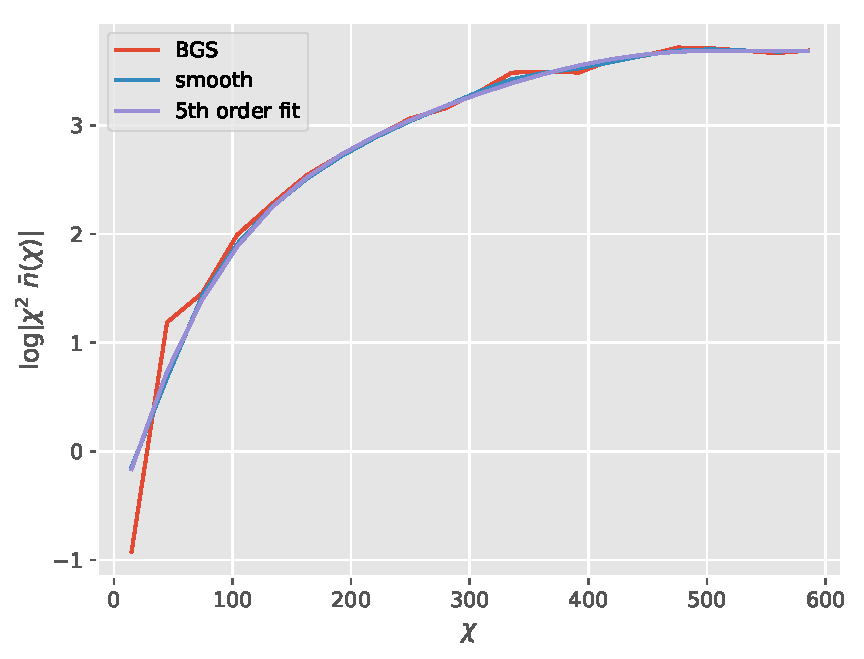
\includegraphics[scale=0.55]{BGS_nx.pdf}
    \caption{The radial selection function for the DESI BGS survey, as estimated from a HOD populated mock given parameters found from the GAMA survey.}
    \label{fig:nx}
\end{figure}
\begin{figure}
    \centering
    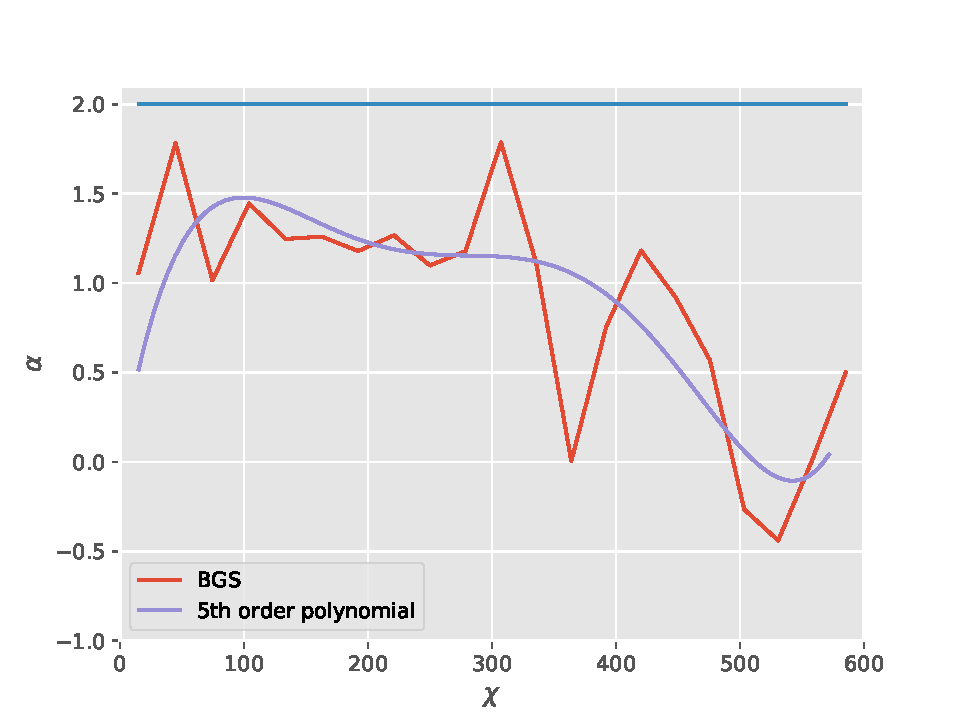
\includegraphics[scale=0.55]{BGS_alpha.pdf}
    \caption{This figure shows $\alpha(s)$ for the DESI BGS survey.  As $\alpha$ is positive to $z=0.175$, the RSD-selection mixing causes a cancellation of finite-angle effects for the majority of the survey.  The application of FKP weighting will further amplify the volume where $\alpha(s)$ is small.}
    \label{fig:alpha}
\end{figure}
\begin{figure*}
    \centering
    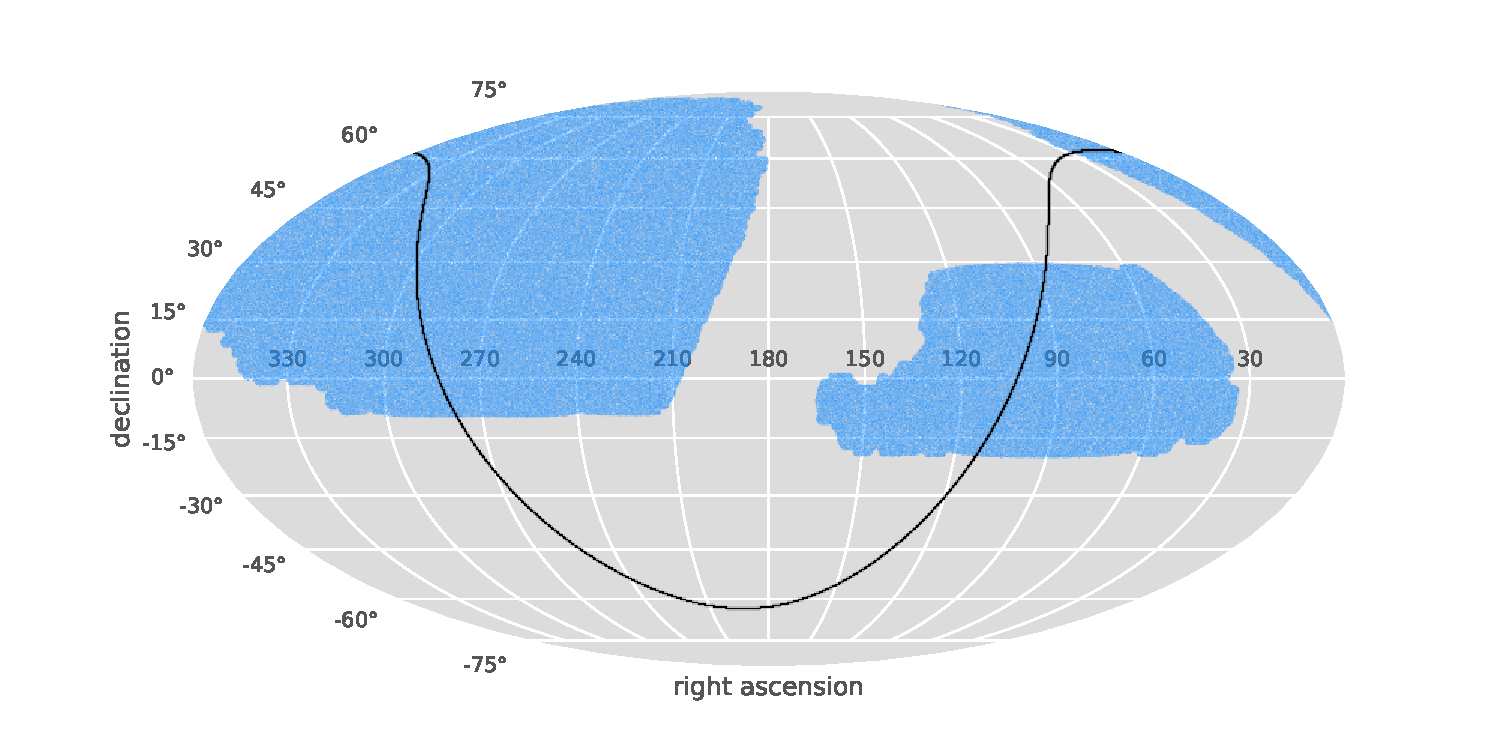
\includegraphics[scale=0.75]{footprint.pdf}
    \caption{DESI footprint: in this paper we consider the Bright Galaxy Survey.  As a close to sample variance limited sample at low redshift, this is likely the future survey for which the effects we consider will be largest.  In principle, local peculiar velocity surveys and, in particular, sample variance cancellation analyses will likely be unable to neglect the effects we consider.}
    \label{fig:footprint}
\end{figure*}

We now consider the impact of the survey selection on the estimated $\hat F_{j_1 j_2 J}(k)$; Typically, this a product of a binary angular mask and a radial selection, which is optimised by the application of FKP weights: $1/(1 + \bar n P)$ per galaxy.  We allow for a radial selection that varies across the sky and show the RSD-selection mixing -- in linear theory, as parameterised by e.g. $\alpha(s_1)$ -- simply multiplies the applied volume weighting.  
Initially, 
\begin{align}
&\avg{\hat{F}_{j_1 j_2 J}(k)} = \int_{\boldsymbol {\hat s}_1, \boldsymbol {\hat s}_2, \boldsymbol {s}} 
\ j_J(ks) \ T^{*}_{j_1 j_2 J}(\blacktriangle) \ W^{+-}(\vb{s}, \vb{d}) \ \xi(\vb{s}_1,\vb{s}_2) \notag \\
 &=
 (4 \pi)^{3/2} \ (-1)^{\ell_1} \ i^{-n} \ \tilde \beta^n_{\ell_1 \ell_2} \notag \\ 
 &\sum_{L=0}^{\ell_1 + \ell_2} (-i)^L \sqrt{\frac{2L+1}{(2\ell_1 +1)(2 \ell_2 +1)}} \tj{\ell_1}{\ell_2}{L}{0}{0}{0} \notag \\ \ & \times \mathcal{H} \left ( \xi^{n}_{L}(s) \ 
 \int_{\boldsymbol{\hat s}_1, \boldsymbol{\hat s}_2, \boldsymbol{\hat s} | s} T_{j_1 j_2 J}(\blacktriangle) \ T_{\ell_1 \ell_2 L}(\blacktriangle) \ \tilde{W}^{+-}(\boldsymbol s, \boldsymbol d) \right ) 
\end{align}
for a (weighted) response to pairs: 
\begin{align}
W^{+-}(\vb{s},\vb{d}) \equiv W(\vb{s}_1) \ W(\vb{s}_2) 
\end{align}
Here the $(n, \ell_1, \ell_2)$ indexing is a result of the entry of the RSD-selection terms in the original Szalay eqn., i.e. they label three forms for $Q$ which are obtained by applying unit, $\alpha(s_1)$ and $\alpha(s_1) \times \alpha(s_2)$ weighting to $W^{+-}(\boldsymbol{s}, \vb{d})$ in the integral; we therefore define $\tilde W^{n \ +-}_{\ell_1, \ell_2} \equiv \alpha^{n}_{\ell_1, \ell_2}(s_1, s_2) \ W^{+-}(\boldsymbol s, \boldsymbol d)$.  Note the artificial pair response of the survey mask breaks the orthogonality of the transform and produces a product of Tripolar Spherical harmonics, which has a Clebsch-Gordan expansion given by V162(17) for $(L', M', L'', M'', L, M) = \boldsymbol 0$ and $(\lambda', \lambda'', \lambda) = ({\ell}'_1, \ell''_1, \ell_1)$.  Schematically, 
\begin{equation}
T_{j_1 j_2 J}(\blacktriangle) \ T_{\ell_1 \ell_2 L}(\blacktriangle) = B^{p_1 p_2 P}_{j_1 j_2 J \ \ell_1 \ell_2 L} \ T_{p_1 p_2 P}(\blacktriangle),  
\end{equation}
where a sum over repeated indices is implied.  Starting with $B$ as given by V162(18) and the indices specified above, using V357(1) and V299(1), this is 
\begin{align}
&B^{p_1 p_2 P}_{j_1 j_2 J \ \ell_1 \ell_2 L}
= \sqrt{\frac{ (2 \ell_1 + 1) (2 j_1 + 1) (2 \ell_2 + 1)(2 j_2 + 1)}{(4 \pi)^3}} \notag \\
& \qquad \qquad \qquad \times \sqrt{(2 L + 1)(2 J + 1)} 
\ C^{p_1 0}_{\ell_1 0 j_1 0} 
\ C^{p_2 0}_{\ell_2 0 j_2 0}
\ C^{P   0}_{L      0 J   0} \notag \\
& \qquad \qquad \qquad \times 
\nj{\ell_1}{j_1}{p_1}{\ell_2}{j_2}{p_2}{L}{J}{P} \notag \\
\end{align}
A given $C^{p_1 0}_{\ell_1 0 j_1 0}$ is non-zero only if $(\ell_1 + j_1 + p_1)$ is even, while the triads specified by every row and column of the Wigner-9j symbol must satisfy the triangular inequalities.  Therefore 
\begin{align}
\avg{\hat{F}_{j_1 j_2 J}(q)} =& (4 \pi)^{3/2} \ (-1)^{\ell_1} \ i^{-n} \ \tilde \beta^n_{\ell_1 \ell_2} \notag \\ 
&\times \sum_{L=0}^{\ell_1 + \ell_2} (-i)^L \sqrt{\frac{2L+1}{(2\ell_1 +1)(2 \ell_2 +1)}} \tj{\ell_1}{\ell_2}{L}{0}{0}{0} \notag \\ \ & \times B^{p_1 p_2 P}_{j_1 j_2 J \ \ell_1 \ell_2 L} \ \mathcal{H} \left( \xi^{n}_{L}(s) \ Q^{n}_{\ell_1 \ell_2 \ p_1 p_2 P}(s) \right ) ,
\end{align}
for 
\begin{equation}
Q^{n}_{\ell_1 \ell_2 \ p_1 p_2 P}(s) = \int_{\blacktriangle | s} \ \tilde W^{n \ +-}_{\ell_1, \ell_2}(\boldsymbol s, \boldsymbol d) \ T_{p_1 p_2 P}(\blacktriangle).
\end{equation}
Note that the sum over $L$ is not infinite, as has been found in studies that assume the local plane-parallel approximation.  With respect to $(p_1, p_2, P)$, there are fourteen allowed triplets in the absence of selection and thirty-five with selection effects;  These are shown in Fig. \ref{fig:qs};  However, the $B$ prefactor strongly downweights the majority of these terms.  We note that perhaps the most natural step is to determine the coefficients of $W^{+-}$ in the full $j_P(ks) \ T_{p_1 p_2 P}(\blacktriangle)$ basis, resulting in an analytically solvable integral of three Bessel functions in eqn. (30) --  see F4 of Castorina and White (2017);  Again the explicit Hankel transform of the mask may be achieved with FFTlog, the efficiency of which make it somewhat unclear that this step is advantageous over eqn.~(30).         

In the small-separation limit, when $T(\blacktriangle)$ reduces to a simple rescaling of a Legendre polynomial, these multipoles reduce to a rescaling of those defined by Wilson et al. (2017); This makes it clear that there is an error in applying the results of a local plane-parallel approximation to pairs of large $s$.  This is perhaps evidenced by the higher-order $RR$ multipoles estimated by Beutler et al. (2017) -- these are larger for the NGC than the SGC, which comprises half of the area.  Wilson et al. (2017) advocated  a Monte-Carlo evaluation that pair counted a large random catalogue spanning the survey geometry, but this work presents a more efficient approach.  

The relevant mask is that which has been averaged by all operations that leave the cosmological dependence of $\xi_s(\boldsymbol s_1, \boldsymbol s_2)$ invariant;  In particular, global rotations about the observer.  Only the mask remaining after projection of $W^{+-}(\boldsymbol{s}, \vb{d})$ onto the rank-zero Tripolar Spherical Harmonics alters the expectation then, the remainder of the degrees of freedom are simply washed out by the applied averaging.  This projected mask is invariant under global rotations about the origin and represented by a rank-zero irreducible tensor.  To exploit this, if $\tilde W^{n \ +-}_{\ell_1 \ell_2}(\boldsymbol{s}, \vb{d})$ is expanded in the coefficients of a Spherical Harmonic transform for each $s_1, s_2$ then 
\begin{align}
\tilde W^{n \ +-}_{\ell_1 \ell_2}(\boldsymbol{s}, \vb{d}) &= \sum_{\ell m} \sum_{\ell' m'} a_{\ell m}(s_1) \ a_{\ell' m'}(s_2) \ Y_{\ell m}(\boldsymbol {\hat s}_1) \ Y_{\ell' m'}(\boldsymbol {\hat s}_2) \notag \\ 
& = \sum_{\ell m} a_{\ell m}(s_1) \ a^{*}_{\ell m}(s_2) \ Y_{\ell m}(\boldsymbol {\hat s}_1) \ Y^{*}_{\ell m}(\boldsymbol {\hat s}_2),
\end{align}
\begin{figure}
    \centering
    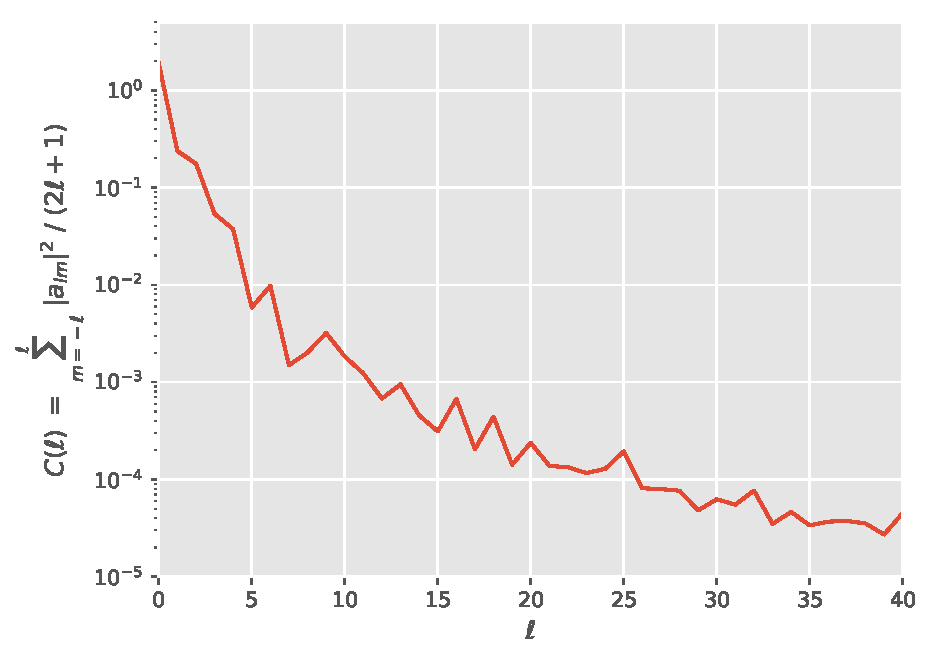
\includegraphics[scale=0.5]{desi_Cls.pdf}
    \caption{This figure shows the $a_{\ell m }$ expansion of the BGS footprint to be rapidly convergent, with $\ell \leq 5$ likely to be sufficient; this will be an ever better approximation for future surveys.}
    \label{fig:Cls}
\end{figure}
\begin{figure}
    \centering
    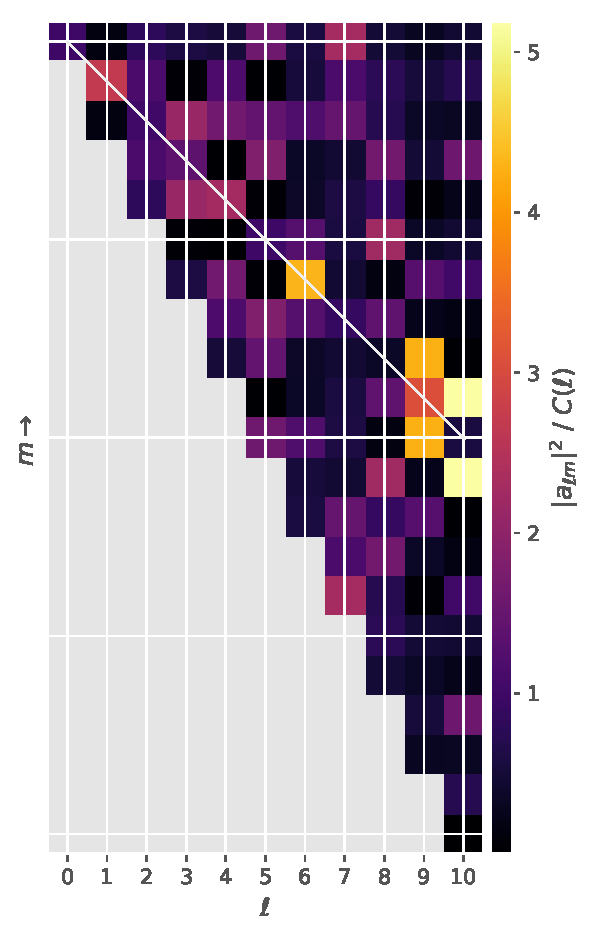
\includegraphics[scale=0.75]{desi_alms.pdf}
    \caption{The variance of the low-order $a_{\ell m}$ for the DESI BGS survey; $m$ increases rising up through the figure.  Together with Fig. (5), this shows that the relevant expressions may be evaluated when only a handful of terms are retained for the survey footprint.}
    \label{fig:alms}
\end{figure}
\begin{figure}
    \centering
    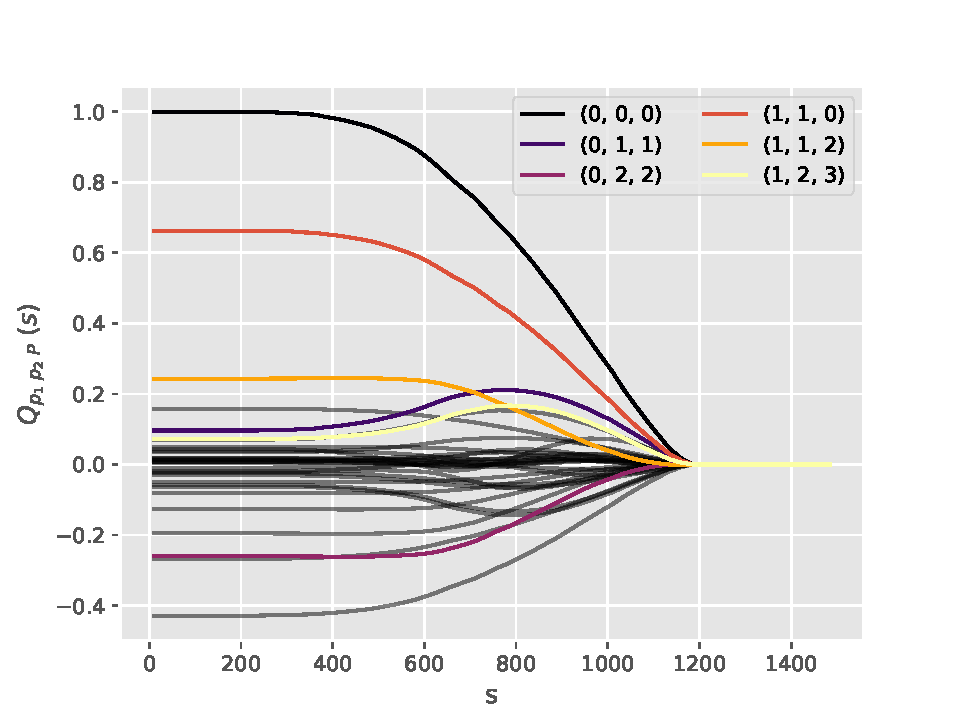
\includegraphics[scale=0.55]{Qs.pdf}
    \caption{The thirty five window function moments required to forward model the spectral moments.}
    \label{fig:qs}
\end{figure}
where the latter follows by analogy to e.g. the analysis of the Cosmic 
Microwave Background, i.e. if there is to be an invariance under global rotation then only the $(\ell', m') = (\ell, -m)$ terms survive;  We prove this in Appendix B.  We expect a small number of such maps as a function of redshift to be sufficient as $\bar n$ is typically a slowly varying function across the redshift divisions adopted by current surveys;  Linear interpolation between these should suffice.  While a few $a_{\ell m }(s)$ should dominate for typical survey footprints, especially for future surveys of increasingly large area;  We examine this for the DESI BGS survey in \S xx.  This approach is the natural limit of those currently considered as both FFT methods and pair counting are unlikely to be practical for the volumes surveyed by future full-sky surveys at moderate redshifts.

Moreover, as the residual mask is invariant under global rotations, we can imagine rotating any pair of randoms into a common plane -- as was the case for the galaxy correlation function.  A further rotation in the plane allows for the enforcement that $\boldsymbol{\hat} s$ lies along the $x$ axis in a spherical coordinate system.  Therefore $Q^{n}_{\ell_1 \ell_2 \ p_1 p_2 P}(s)$ may be evaluated as a two-dimensional integral in the equatorial plane:
\begin{equation}
Q^{n}_{\ell_1 \ell_2 \ p_1 p_2 P}(s) = %\int_{\fatslash} \ s_1^{2} \ ds_1 d\Omega_{\boldsymbol{\hat s}_1} \ d\Omega_{\boldsymbol{\hat s}} \ W_{xx}(s, s_1, \boldsymbol {\hat s}, \boldsymbol {\hat s}_1) \notag \\
\int^{\pi/2}_0 d^2 \phi \ W^{+-}(s_1, s_2) \cos (2 n_1 \phi_1) \cos (2 n_2 \phi_2) 
%&\simeq 
%\left ( \frac{4 \pi}{N_{\rm{pix}}} \right )^2
%\int_{\fatslash} s_1^2 \ ds_1 \sum_{i \in \boldsymbol{\hat s}_1} \sum_{j \in \boldsymbol{\hat s}} \ W_{xx}(s, s_1, \boldsymbol {\hat s}, \boldsymbol {\hat s}_1) 
\end{equation}
where
\begin{align}
s_1 &= s \times \sin(\phi_2) / \sin(\phi_2 - \phi_1) \notag \\ 
s_2 &= s \times \sin(\phi_1) / \sin(\phi_2 - \phi_1)
%    W_{xx}(s, s_1, \boldsymbol {\hat s}, \boldsymbol {\hat s}_1) \equiv \sum_{\ell m} a_{\ell m}(s_1) \ a^{*}_{\ell m}(s_2) \ %\mathds{1}
%    \ Y_{\ell m}(\boldsymbol {\hat s}_1)
%    \ Y_{\ell p_1 m}(\boldsymbol {\hat s}_1)
%    \ Y^{*}_{\ell m}(\boldsymbol {\hat s}_2)
%    \ Y_{\ell p_2 m}(\boldsymbol {\hat s}_2)
\end{align}
%where $\boldsymbol{s_2}(s, s_1, \boldsymbol {\hat s}, \boldsymbol {\hat s}_1)$ is to be understood as implicitly defined.  
and similarly for a $\sin$ basis analogue; Here we choose the coordinate scheme employed by Szapudi (case A).  With 
\begin{equation}
    W^{+-}(s_1, s_2) = \sum_{\ell m} \ a_{\ell m}(s_1) \ a^{*}_{\ell m}(s_2) \ \mathcal{!!}_{\ell m}^2 \ e^{i m (\phi_1 - \phi_2)}.  
\end{equation}
Where $Y_{\ell m}(\pi /2, \phi) = (-1)^{(\ell+m)/2} \ \mathcal{!!}_{\ell m} \ \exp( i m \phi)$ if $(\ell + m)$ is even and zero otherwise;  $\mathcal{!!}_{\ell m}$ is a prefactor to be found in V158(2), it is invariant under $m \mapsto -m$. 
%The planar constraint yields a further restriction on the allowed terms: $(\ell + m)$ must be even for a given $Y_{\ell m}$ to be non-zero for $\theta = (\pi / 2)$; while the evaluation of the non-zero terms reduces to V158(2).  This allows for both a reduction in memory -- the 2D matrix representing $Y_{\ell m}$ for the set of pixels and $(\ell, m)$ is reduced to that where $(\ell + m)$ is even -- and a stride length of two for sums over $m$.  
With this final optimisation, an evaluation of all $Q$ takes roughly xxx minutes for a single core at one degree resolution.

%\section{Bispectrum}

\section{Gaussian covariance of the power spectrum} In this section, we derive analagous expressions for the Gaussian covariance of the estimator:
\begin{align}
&\avg{\hat{F}_{j_1 j_2 J}(k) \ \hat{F}_{j_1' j_2' J'}(k')} - \avg{\hat{F}_{j_1 j_2 J}(k)} \avg{\hat{F}_{j_1' j_2' J'}(k')}  = \notag \\
&
\int_{\boldsymbol{\hat s}_1, \boldsymbol{\hat s}_2, \boldsymbol{s}}
\int_{\boldsymbol{\hat s}_1', \boldsymbol{\hat s}_2', \boldsymbol{s}'}
j_J(ks) \ j_{J'}(k' s') \ T^{*}_{j_1 j_2 J}(\blacktriangle) \ T^{*}_{j_1' j_2' J'}(\blacktriangle') \notag \\
& \qquad \qquad \qquad \qquad \times 
W^{++--}(\boldsymbol{s}, \boldsymbol{d}, \boldsymbol{s'}, \boldsymbol{d'})
\ \left \langle \delta_1 \delta_2 \delta_{1}' \delta_{2}' \right \rangle.
\end{align}
Given Wick's theorem for a Gaussian field, 
\begin{equation}
\left \langle \delta_1 \delta_2 \delta_{1}' \delta_{2}' \right \rangle = 
\left \langle \delta_1 \delta_{2} \right \rangle
\left \langle \delta_1' \delta_{2}' \right \rangle
+
\left \langle \delta_1 \delta_{1}' \right \rangle
\left \langle \delta_2 \delta_{2}' \right \rangle + \left \langle \delta_1 \delta_{2}' \right \rangle
\left \langle \delta_2 \delta_{1}' \right \rangle,
\end{equation}
this is
\begin{align}
& \int_s \int_{s'} s^2 \ s'{}^2 \ j_J(ks) \ j_{J'}(k' s') 
\int_{\boldsymbol{\hat s}_1, \boldsymbol{\hat s}_2, \boldsymbol{\hat s}, \boldsymbol{\hat s}_1', \boldsymbol{\hat s}_2', \boldsymbol{\hat s}' | s, s'}
\notag \\
& \qquad \times \ T_{j_1 j_2 J}(\blacktriangle) \ T_{j_1' j_2' J'}(\blacktriangle') \ W^{++--}(\boldsymbol{s}, \boldsymbol{d}, \boldsymbol{s'}, \boldsymbol{d'})
\ \notag \\
& \qquad \times \ \left [ \xi_s(\boldsymbol {s}_1, \boldsymbol {s}_1') \ \xi_s(\boldsymbol {s}_2, \boldsymbol {s}_2') + \ (1' \leftrightharpoons 2') \right ] 
 \notag \\
&= \int_{s, s'}
s^2 \ s'{}^2 \ j_J(ks) \ j_{J'}(k' s') \ \int_{u, v} u^2 v^2 \ \xi^{(n)}_L(u) \ \xi^{(n')}_{L'}(v) \notag \\ 
& \qquad \times \left [  P_{j_1 j_2 J \  j_1' j_2' J'}^{\ell_1 \ell_2 L \ \ell_1' \ell_2' L'}(s, s', u, v) + \ (1' \leftrightharpoons 2') \right ].
\end{align}
As this configuration of two pairs can be fully described by eight vectors, four of which have unit length, the volume element for a configuration is $s^2 \ s^2{}' \ u^2 \ v^2 \ d^4s \ d^8 \Omega$; the $\sqrt{g(u,v)} = u^2 \ v^2$ then results from making the sum over $u,v$ within the integrals in eqn. (36) explicit. 
For 
\begin{align}
&P_{j_1 j_2 J \  j_1' j_2' J'}^{\ell_1 \ell_2 L \ \ell_1' \ell_2' L'}(s, s', u, v) = \notag \\ &\int_{\blacktriangle, \blacktriangle', \boldsymbol{\hat u}, \boldsymbol{\hat v} | s, s', u = |\boldsymbol s_1 - \boldsymbol s_1'|, v = |\boldsymbol s_2 - \boldsymbol s_2'|}
\widetilde{\widetilde W} {}^{++--}(\boldsymbol{s}, \boldsymbol{d}, \boldsymbol{s'}, \boldsymbol{d'}) \notag \\ 
& \times T_{j_1 j_2 J}(\blacktriangle) \ 
T_{j_1' j_2' J'}(\blacktriangle') \ T_{\ell_1 \ell_2 L}(\boldsymbol{\hat s}_1, \boldsymbol{\hat s}_1', \boldsymbol{\hat u})
\ T_{\ell_1' \ell_2' L'}(\boldsymbol{\hat s}_2, \boldsymbol{\hat s}_2', \boldsymbol{\hat v}).
\end{align}
Here $(1' \leftrightharpoons 2')$ indicates that the analagous function is to be obtained with the same integral as that for $P$, but with $\boldsymbol s_1'$ and $\boldsymbol s_2'$ swapped in the definition of $\boldsymbol{u}$ and $\boldsymbol{v}$.  In this form (where we have dropped various coefficients, e.g. $\beta^{n}_{\ell_1 \ell_2}$), the cosmology dependence has been isolated such that the evaluation of the covariance is straightforward if $P$ and the additional cross may be estimated.  While estimates of the covariance for the binned multipoles may be obtained by a replacement with $\bar j_L(ks)$, where a bar indices a top-hat average weighted by a mode counting $k^2$ factor.

To this end, the rank-zero product of the configuration and cross-configuration harmonics, $T_{j_1 j_2 J}(\blacktriangle) \ 
T_{j_1' j_2' J'}(\blacktriangle') \ T_{\ell_1 \ell_2 L}(\boldsymbol{\hat s}_1, \boldsymbol{\hat s}_1', \boldsymbol{\hat u})
\ T_{\ell_1' \ell_2' L'}(\boldsymbol{\hat s}_2, \boldsymbol{\hat s}_2', \boldsymbol{\hat v})$, has a series expansion in the rank-zero Octupolar Spherical harmonics: 
\begin{align}
O(\blacktriangle, \blacktriangle', \times) \equiv & \ \ \{ \{ \{ Y_{\ell_1} \otimes Y_{\ell_2} \}_{\ell_{12}} \otimes \{ Y_{\ell_3} \otimes Y_{\ell_4} \}_{\ell_{34}} \}_{\ell_{1234}} \notag \\ 
& \otimes
\{ \{ Y_{\ell_5} \otimes Y_{\ell_6} \}_{\ell_{56}} \otimes \{ Y_{\ell_7} \otimes Y_{\ell_8} \}_{\ell_{78}} \}_{\ell_{5678}} \}_{00} \notag \\
= & \sum \mathcal{C}^{00} \ 
\ Y_{\ell_1 m_1}(\boldsymbol{\hat s}_1)
\ Y_{\ell_2 m_2}(\boldsymbol{\hat s}_2)
  Y_{\ell_5 m_5}(\boldsymbol{\hat s})
\notag \\ 
& \qquad \qquad
\ Y_{\ell_3 m_3}(\boldsymbol{\hat s}_1')
\ Y_{\ell_4 m_4}(\boldsymbol{\hat s}_2')
\ Y_{\ell_6 m_6}(\boldsymbol{\hat s}')
\notag \\ 
& \qquad \qquad
\ Y_{\ell_7 m_7}(\boldsymbol{\hat u})
\ Y_{\ell_8 m_8}(\boldsymbol{\hat v}).
\end{align}
where 
\begin{align}
\mathcal{C}^{LM} = 
&\ C^{LM}_{\ell_{1234} m_{1234} \ell_{5678} m_{5678}} 
\ C^{\ell_{1234} m_{1234}}_{\ell_{12} m_{12} \ell_{34} m_{34}}
\ C^{\ell_{5678} m_{5678}}_{\ell_{56} m_{56} \ell_{78} m_{78}}\notag \\
& 
\times 
C^{\ell_{12}   m_{12}}_{\ell_1 m_1 \ell_2 m_2} 
\ C^{\ell_{34}   m_{34}}_{\ell_3 m_3 \ell_4 m_4}
\ C^{\ell_{56}   m_{56}}_{\ell_5 m_5 \ell_6 m_6}
\ C^{\ell_{78}   m_{78}}_{\ell_7 m_7 \ell_8 m_8}
\end{align}
and 
%Formally, the projection onto a rank-zero irreducible tensor implies
\begin{align}
    \widetilde{\widetilde W}(\boldsymbol{s}, \vb{d}, \vb{s}', \vb{d}') =    
    & \sum_{\ell_1 m_1} \sum_{\ell_2 m_2} \sum_{\ell_3 m_3} \sum_{\ell_4 m_4} \notag \\ 
    &a_{\ell_1 m_1}(s_1) \ a_{\ell_2 m_2}(s_2) \ a_{\ell_3 m_3}(s_1') \ a_{\ell_4 m_4}(s_2')\ \notag \\ 
    &Y_{\ell_1 m_1}(\boldsymbol {\hat s}_1) \ Y_{\ell_2 m_2}(\boldsymbol {\hat s}_2) \
    Y_{\ell_3 m_3}(\boldsymbol {\hat s}_1') \
    Y_{\ell_4 m_4}(\boldsymbol {\hat s}_2').
    %\notag \\  
    %&= \frac{(-1)^{\ell_{12}'}}{\sqrt{2 \ell_{12}' + 1}} \sum_{m_{12'}} (-1)^{- m_{12}'} \ C^{\ell_{12}' m_{12}'}_{\ell_1 m_1 \ell_2 m_2} \ C^{\ell_{12}' - m_{12}'}_{\ell_3 m_3 \ell_4 m_4} \notag \\ 
    %&a_{\ell_1 m_1}(s_1) \ a_{\ell_2 m_2}(s_2) \ a_{\ell_3 m_3}(s_3) \ a_{\ell_4 m_4}(s_4)\ \notag \\ 
    %&
    %Y_{\ell_1 m_1}(\boldsymbol {\hat s}_1) \ Y_{\ell_2 m_2}(\boldsymbol {\hat s}_2) \ 
    %Y_{\ell_3 m_3}(\boldsymbol {\hat s}_3) \
    %Y_{\ell_4 m_4}(\boldsymbol {\hat s}_4),
\end{align}
%where the latter illustrates the restriction of isotropy on the sums when constracted against a rank-zero tensor, i.e. each input $(\ell, m)$ must couple correctly to give an allowed $\ell_{12}$ and $m_{12}$ -- the specific restriction being dependent on a given $O$; Enforcement of this condition aids the resolution of isotropy if a finite pixelisation is employed.  Therefore, we have as fundamental constructs to be evaluated:
This is the most succinct representation of the independent degrees of freedom of the configuration that are invariant under rotation about the observer.  As for any N-polar Spherical Harmonic, these are simply constructed by products of Clebsch-Gordan coefficients that couple two momenta to a third in order to progressively build that associated to $(L, M)$, in a given coupling scheme.  These are related to the alternatives schemes by Wigner-j symbols, which are further reducible given the $(L,M) = (0,0)$ constraint.  This global isotropy about the observer further ensures the final coupling coefficient must be $C^{00}_{\ell_{1234} \ m_{1234} \ \ell_{5678} \ m_{5678}}$, which places the restriction: $\ell_{1234} = \ell_{5678}$ and $m_{1234}~=~-m_{5678}$; see V248(1).
%The resulting product of rank-zero Hexapolar harmonics may then be reduced to a single Hexapolar harmonic given the N-polar Clebsch-Gordan expansion derived in Appendix B.  This is proportional to
%\begin{align}
%& \quad \nj{\ell_1 '}{\ell_1 ''}{j_1}{\ell_2 '}{\ell_2 ''}{j_2}{\ell_{12} '}{\ell_{12} ''}{j_{12}}  
%\times \nj{\ell_3 '}{\ell_3 ''}{j_3}{\ell_4 '}{\ell_4 ''}{j_4}{\ell_{34} '}{\ell_{34} ''}{j_{34}}
%\notag \\
%&\times \nj{\ell_5 '}{\ell_5 ''}{j_5}{\ell_6 '}{\ell_6 ''}{j_6}{\ell_{56} '}{\ell_{56} ''}{j_{56}}
%\times \nj{\ell_{56} '}{\ell_{56} ''}{j_{56}}{\ell_{1234} '}{\ell_{1234} ''}{j_{1234}}{L '}{L ''}{J}
%\end{align}
%\emph{To be confirmed, I'm not sure how the internal couplings work out just yet}.  Therefore $W^{++--}$ is again projected, but onto a rank-zero Hexapolar Spherical Harmonic.  

Analogously to the Clebsch-Gordan coefficient $B^{p_1 p_2 P}_{j_1 j_2 J \ \ell_1 \ell_2 L}$ in the two-point expectation, the coefficient of the Octupolar series expansion:  
\begin{align}
    &\mathcal{B}_{\ j_1 j_2 J \ j_1' j_2' J' \ \ell_1 \ell_2 L \ \ell_1' \ell_2' L'}^{\ p_1 \ p_2 \ p_{12} \ p_3 \ p_4 \ p_{34} \ p_5 \ p_6 \ p_{56} \ p_7 \ p_8 \ p_{78} \ p_{5678}} = \notag \\
    & (-1)^{j_1     + j_2     + J}
      (-1)^{j_1'    + j_2'    + J'}
      (-1)^{\ell_1  + \ell_2  + L}
      (-1)^{\ell_1' + \ell_2' + L'}
      \notag \\
     & \tilde B(j_1,  \ell_1,  p_1) \
      \tilde B(j_2,  \ell_1', p_2) \
      \tilde B(j_1', \ell_2,  p_3) \ 
      \tilde B(j_2', \ell_2', p_4) \notag \\
    & \sum_{o, o', n, n', m} \mathcal{C}^{00} \ C^{p_1 m_1}_{j_1 o_1 \ell_1 n_1} \
        C^{p_2 m_2}_{j_2 o_2 \ell_1' n_1'} \ 
        C^{p_3 m_3}_{j_1' o_1' \ell_2 n_2}
        C^{p_4 m_4}_{j_2' o_2' \ell_2' n_2'}
        \notag \\
    &  \qquad \qquad \tj{j_1}{j_2}{J}{o_1}{o_2}{m_5}
    \tj{j_1'}{j_2'}{J'}{o_1'}{o_2'}{m_6} \notag \\ 
    &  \qquad \qquad \tj{\ell_1}{\ell_2}{L}{n_1}{n_2}{m_7}
    \tj{\ell_1'}{\ell_2'}{L'}{n_1'}{n_2'}{m_8} \notag \\
    & \ \ \qquad \qquad 
    \delta^{K}_{p_5 J} \
    \delta^{K}_{p_6 J'} \
    \delta^{K}_{p_7 L} \ 
    \delta^{K}_{p_8 L'},
\end{align}
where
\begin{equation}
    \tilde B(j, \ell, p) = \sqrt{\frac{(2 j + 1)(2 \ell + 1)}{4 \pi (2p+1)}} \ C^{p0}_{j0 \ell 0}, 
\end{equation}
relates the fundamental independent constructs:
\begin{align}
&\mathcal{P}_{p_1 \ p_2 \ p_{12} \ p_3 \ p_4 \ p_{34}\ p_{5} \ p_{6} \ p_{56} \ p_{7} \ p_{8} \ p_{78} \ p_{5678}}(s, s', u, v) = \notag \\ &\int
\ d\Omega_{\boldsymbol{\hat s}_1}
\ d\Omega_{\boldsymbol{\hat s}_2}
\ d\Omega_{\boldsymbol{\hat s}}
\ d\Omega_{\boldsymbol{\hat s}_1'}
\ d\Omega_{\boldsymbol{\hat s}_2'}
\ d\Omega_{\boldsymbol{\hat s}'}
\ d\Omega_{\boldsymbol{\hat u}}
\ d\Omega_{\boldsymbol{\hat v}}
\notag \\ 
& \times 
\widetilde{\widetilde W} {}^{++--}(\boldsymbol{s}, \boldsymbol{d}, \boldsymbol{s'}, \boldsymbol{d'}) \notag \\ 
& \times O_{p_1 \ p_2 \ p_{12} \ p_3 \ p_4 \ p_{34} \ p_{5} \ p_{6} \ p_{56} \ p_{7} \ p_{8} \ p_{78} \ p_{5678}}(\blacktriangle, \blacktriangle {}', \times),
\end{align}
to those needed to evaluate eqns. (33) and (36).  The restrictions placed by $\mathcal{B}$ and the base triplets relevant to RSD ($j, \ell \in \{ 0,1, 2 \}$) determines the allowed sets for $p$.  The restriction on coupled indices is provided solely by $\mathcal{C}^{00}$.  We find only xxx to be non-zero.  \emph{The degrees of freedom are too many for $W^{++--}$, what restrictions does this place?}.  % As $W^{++--}$ is fully described by $(s, \boldsymbol{\hat s}_1, \boldsymbol{\hat s}_2, s', \boldsymbol{\hat s}_1', \boldsymbol{\hat s}_2')$, then $p_5 = p_6 = p_7 = p_8 = 0$, and similarly for the associated $m$s.   

To evaluate the integral, one pair may be assumed to lie in the equatorial plane due to the global isotropy -- with $\boldsymbol{\hat s}$ again along $\boldsymbol{\hat x}$. But the relative orientation of the other is free,  outwith the constraint placed by fixing $u$ and $v$.  Thus this reduces to an evaluation of the planar integral for each sampling of a pair with arbitrary orientation.  We utilise a number of methods to implement this.  

First, we adopt much of the methodology of Gorksi et al. (HEALPix, 2004).  Using Healpy, the sphere is divided into equal area pixels defined hierarchically on rings of constant co-latitude.  The associated Legendre polynomial for each $Y_{\ell m}$ must then be calculated only once per co-latitude ring, which achieves a transition from a $N_{\rm{pix}}^2$ to $N_{\rm{pix}}^{3/2}$ scaling.  The effective angular resolution achieved is approximately $\sqrt{\Omega_{\rm{pix}}} = (\sqrt{\pi / 3} \ / \ n_{\rm{side}})$ for given $n_{\rm{side}}$, but note that the resolution is both anisotropic and inhomogeneous on the sphere;  Given a maximum $\ell$ to be integrated, the necessary resolution is approximately $(1 / \ell)$ in radians.  

Adopting a HEALPix ringed labelling and a $\ell^2 + \ell + m + 1$ integer indexing for the $a_{\ell m}$ satisfying $\ell < \ell_{\rm{max}}$, the required $Y_{\ell m}$ evaluated on the pixelated sphere is represented by a two-dimensional matrix with complex elements; computed once, this is effectively a look-up table for evaluating any factor specified by a given pixel and $(\ell, m)$.  E.g., a product $Y_{\ell' m'}(\boldsymbol{\hat s}_1) \ Y_{\ell m}(\boldsymbol{\hat s}_2)$ is represented by a two-dimensional matrix that may be computed with a (sparse) Kronecker product.  Finally, the double integral over solid angle is achieved by summing the elements of the 2D matrix product.  A neat implementation of the integral when constrained to the equatorial plane is to simply replace the full list of pixels with the sublist of those satisfying $\theta = (\pi / 2)$.  

%As an integral, this is simply a `squared' copy of the two-point algorithm -- being composed of a sum over elements of the (sparse) Kronecker product of a pair of two-dimensional matrices. 
The required selection by $u$ and $v$, together with the internally coupled indices, are unique to the covariance calculation, however; internally coupled indices, e.g. $p_{12}$ have no associated $Y$.  The former is achieved by masking the final Kronecker product according to the $(u,v)$ of each element before summing;  The $1 \leftrightharpoons2$ analogue may be determined in the same manner. \emph{What independent information is $1 \leftrightharpoons2$ measuring, if any?}.    
We make all necessary code available at \url{bccp.berkeley.edu}.
%In the small separation limit, The required weighting is then
%\begin{equation}
%\alpha_{1234} \
%\mathcal{L}_C \
%\mathcal{L}_D \
%\mathcal{L}_E \
%\mathcal{L}_F.
%\end{equation}

% Is there an estimator for $P$ and $R$ that's analagous to jack-knifing?  Randoms as Poisson sampling of a homogeneous density field (in the absence of a radial selection). 

%Possible to reverse it and obtain estimates from randoms in the holes of the survey. 

%\section{Relation to the Spherical-Bessel transform}
%\section{Alcock-Paczynski}
\appendix
\section{RSD symmetries and their representation}
Consider the orthogonality relation employed:
\begin{align}
& \Xi_{j_1 j_2 J}(s) = \int_{\boldsymbol {\hat s}_1, \boldsymbol {\hat s}_2, \boldsymbol {\hat s} | s} \xi_s(s, \blacktriangle) \ T_{j_1 j_2 J}(\blacktriangle). 
\end{align}
This is at first sight an apparent overcounting of the degrees of freedom for the triangle configuration to be described in finite-angle RSD.  This is an artefact of the abstraction adopted by Szapudi (2004), which removes the physical restriction placed on $\blacktriangle$ by $s$, in order to write $\xi_s$ as separable factors of a configuration dependent basis -- the Tripolar Spherical Harmonics -- and solely $s$ dependent coefficients;  Thereby separating the configuration dependence from the (real-space) cosmology.  This basis is complete and has only a finite number of non-zero coefficients, even for large $s$.  

For given $s$, $\boldsymbol{\hat s}_1$ and $\boldsymbol{\hat s}_2$, one finds that $\boldsymbol{\hat s}$
is restricted to lie between $\boldsymbol{\hat s}_1$ and $- \boldsymbol{\hat s}_2$; see Fig. xx.  In linear theory, when $s$ and $\boldsymbol{\hat s}_1$ are fixed, $\xi_s$ is invariant under $D: \boldsymbol{\hat s}_2 \ \mapsto - \boldsymbol{\hat s}_2$ in the absence of RSD-selection mixing, despite this corresponding to unphysical directions for the `separation' vector; this transformation forms an isoceles triangle of which $s_1$ is a cevian, therefore Stewart's theorem yields $s$ for the image of $\boldsymbol{s}_2$.  One may adopt this definition as an analytic continuation of $\xi_s$ for a generalised separation $\boldsymbol{\hat s}$ that spans a hemisphere without restriction; when pair exchange symmetry is employed -- $\xi_s(s, \blacktriangle)$ should be invariant under $1 \rightleftharpoons 2$ -- this is further extended to the full sphere; These two mappings thus partition the sphere in four, with two pairs of equal solid angle.  The generalised separation, $\boldsymbol{\hat s}$, is no longer restricted by $s$, and the three unit direction vectors should be considered independent of both $s$ and each other.  This is the basis of an expansion of the (continued) $\xi_s$ in Tripolar Spherical Harmonic expansion, which require the three vectors to be independent for orthonormality to be applied.

Providing $\alpha$ is an isotropic function, we can retain the analytic continuation in rank-zero Tripolar Spherical harmonics when selection effects are included.  In this case, the expansion coefficients should be held fixed and $T_{\ell_1 \ell_2 L}(\blacktriangle) \mapsto (-1)^{\ell_2} T_{\ell_1 \ell_2 L}(\blacktriangle)$ under $D$ at fixed $\boldsymbol{\hat s}_1$ and $\boldsymbol{\hat s}$; these are invariant for non-selection terms and change sign otherwise.  Irreducible tensors are generally composed of two such components of definite parity, see V62(12).  The analytic continuation of $\xi_s$ corresponds simply to the superposition in this case.  Although the extended $\xi_s$ is then not equal to the true one -- as was the case in the absence of selection effects -- crucially, the coefficients are identical and may be extracted in order to describe the physical space without bias.

The analytic continuation with selection terms has further consequences for the $\xi_s$ symmetries discussed by Szapudi (2004).  In particular, as $\boldsymbol{\hat s}$ and its image under $D$ flip direction under $1 \leftrightharpoons 2$, the generalised $\xi_s$ remains invariant under pair exchange.  It remains both real and invariant under global rotation.



\section{N-polar Spherical Harmonic identities}
\subsection{Proof of eqn. (22)}
Eqn. (22) reduces a double to a single sum on the basis of invariance under global rotation.  To prove this requires extracting the coefficents for an expansion in the rank-zero Bipolar Spherical Harmonics from a product of Spherical Harmonics.  This is  
\begin{align}
&\int d \Omega_1 \ d \Omega_2 \ Y_{\ell_1 m_1}(\Omega_1) \ Y_{\ell_2 m_2}(\Omega_2) \ \{ Y_{\ell_3} (\Omega_3) \otimes Y_{\ell_4} (\Omega_4) \}_{00}^{*} \notag \\
& = \sum_{m_3 m_4} C^{00}_{\ell_3 m_3 \ell_4 m_4} \int d \Omega_1 \ d \Omega_2 Y_{\ell_1 m_1}(\Omega_1) \ Y_{\ell_2 m_2}(\Omega_2) \ \notag \\
& \qquad \times Y_{\ell_3, m_3}^{*} (\Omega_3) \ Y_{\ell_4, m_4}^{*} (\Omega_4) \notag \\
& = \sum_{m_3 m_4} C^{00}_{\ell_3 m_3 \ell_4 m_4} \delta^{K}_{\ell_1 \ell_3} 
\delta^{K}_{\ell_2 \ell_4} 
\delta^{K}_{m_1 m_3}
\delta^{K}_{m_2 m_3} \notag \\ 
& = C^{00}_{\ell_1 m_1 \ell_2 m_2} = \frac{(-1)^{\ell_1 - m_1}}{\sqrt{2 \ell + 1}} \delta_{\ell_1 \ell_2} \delta_{m_1 -m_2},
\end{align}
where $C^{JM}_{j_1 m_1 j_2 m_2}$ are the Clebsch-Gordan coefficients.  This proves the $(\ell, m) = (\ell', -m')$ assumed by analogy with the analysis of the Cosmic Microwave Background.  
%For the Hexapolar case required for the covariance calculation, this is 
%\begin{align}
%&\int d^{6} \Omega \ Y_{\ell_1 m_1}(\Omega_1) \ Y_{\ell_2 m_2}(\Omega_2) \ Y_{\ell_3 m_3}(\Omega_3) \ Y_{\ell_4 m_4}(\Omega_4) \notag \\ 
%& \qquad \times \{ \{ \{ Y_{\ell_1'} \otimes Y_{\ell_2'} \}_{\ell_{12}'} \otimes \{ Y_{\ell_3'} \otimes Y_{\ell_4'} \}_{\ell_{34}'} \}_{\ell_{1234}'} \otimes \{ Y_{\ell_5'} \otimes Y_{\ell_6'} \}_{\ell_{56}'} \}_{00} \notag \\
%& = \frac{(-1)^{\ell_{12}'}}{\sqrt{2 \ell_{12}' + 1}} \sum_{m_{12'}} (-1)^{- m_{12}'} \ C^{\ell_{12}' m_{12}'}_{\ell_1 m_1 \ell_2 m_2} \ C^{\ell_{12}' - m_{12}'}_{\ell_3 m_3 \ell_4 m_4}.
%\end{align}

\subsection{Clebsch-Gordan coefficients}
Schematically,
\begin{equation}
    N' \times N'' \mapsto N
\end{equation}
where $N$ is to represent a given N-polar spherical harmonic.  The initial product is
\begin{equation}
    \sum _{m' \rm{s}, \ m'' \rm{s}} \ \mathcal{C}^{L' M'} \ \mathcal{C}^{L'' M''} \prod_i^{N} Y_{\ell_i ' m_i'} (\Omega_i) \ Y_{\ell_i '' m_i''}(\Omega_i),
\end{equation}
where the sum includes internal couplings but not the outer.  Expanding each $\Omega_i$ dependent product using V144(9), this is
\begin{align}
    &\sum _{m' \rm{s}, \ m'' \rm{s}} \ \mathcal{C}^{L' M'} \ \mathcal{C}^{L'' M''} \notag \\ 
    & \times \ \prod_i^{N} \sum_{\ell_i m_i}
    \ \sqrt{\frac{(2 \ell_i' + 1)(2 \ell_i '' +1)}{4 \pi (2 \ell_i + 1)}} 
    \ \cg{\ell_i}{0}{\ell_i'}{0}{\ell_i''}{0}
    \ \cg{\ell_i}{m_i}{\ell_i'}{m_i'}{\ell_i''}{m_i''} 
    \ Y_{\ell_i m_i}(\Omega_i).
\end{align}
A weighted integral with a kernel consisting of the complex conjugate of a N-polar Spherical Harmonic gives the required coefficient:
\begin{align}
&\sum_{m' \rm{s}, \ m'' \rm{s}, \ o \rm{s}}    
\mathcal{C}^{L' M'} \ 
\mathcal{C}^{L'' M''} \ 
\mathcal{C}^{J O} \ 
\notag \\ 
& \times \ \prod_i^{N} \sum_{\ell_i m_i}
    \ \sqrt{\frac{(2 \ell_i' + 1)(2 \ell_i '' +1)}{4 \pi (2 \ell_i + 1)}} 
    \ \cg{\ell_i}{0}{\ell_i'}{0}{\ell_i''}{0}
    \ \cg{\ell_i}{m_i}{\ell_i'}{m_i'}{\ell_i''}{m_i''} \notag \\
    & \int d^N \Omega \ Y_{\ell_i m_i}(\Omega_i) \ Y_{j_i o_i}(\Omega_i).
\end{align}
As $\int d^N \Omega \ Y_{\ell_i m_i}(\Omega_i) \ Y_{j_i o_i}(\Omega_i) = \delta^{K}_{\ell_i j_i} \delta^{K}_{m_i o_i}$, the final result is 
\begin{align}
    & \sum_{JO} 
    \ C^{JO}_{L' M' L'' M''} \notag \\ 
    & \times 
    C^{JO}_{L' M' L'' M''}
    \ \mathcal{C}^{L' M'}
    \ \mathcal{C}^{L'' M''}
    \notag \\ 
    & \times \ \mathcal{C}^{JO} \ \prod_i^{N} \cg{j_i}{o_i}{\ell_i'}{m_i'}{\ell_i''}{m_i''}
    \notag \\ 
    & \times \prod_i^{N} \sqrt{\frac{(2 \ell_i' + 1)(2 \ell_i '' +1)}{4 \pi (2 j + 1)}} \ \cg{j_i}{0}{\ell_i'}{0}{\ell_i''}{0}.
\end{align}
As a product of two sets of Clebsch-Gordan coefficients in independent coupling schemes that both generate a final $(J,N)$ state, this has a representation in Wigner-j symbols.  The initial pre-factor has been extracted as this is incorporated in the irreducible N-polar basis functions. 

%\section{Useful identities}
%\begin{equation}
%\mathcal{L}_{\ell_1}(\boldsymbol {\hat s} \cdot \boldsymbol{\hat d})  \ \mathcal{L}_{\ell_2} (\boldsymbol {\hat s} \cdot \boldsymbol {\hat d}) = \sum_{L} (2L \ + \ 1) \tj{\ell_1}{\ell_2}{L}{0}{0}{0}^2 \mathcal{L}_L(\boldsymbol {\hat s} \cdot \boldsymbol {\hat d}),
%\end{equation}
%where $L$ satisfies the triangular inequalities. 

\bibliographystyle{mn2e}
\bibliography{main}

\end{document}
